%% LaTeX2e class for student theses
%% sections/content.tex
%% 
%% Karlsruhe Institute of Technology
%% Institute for Program Structures and Data Organization
%% Chair for Software Design and Quality (SDQ)
%%
%% Dr.-Ing. Erik Burger
%% burger@kit.edu
%%
%% Version 1.3.3, 2018-04-17
\chapter{Case study}
\label{ch:case_study}

After we have covered the basic concepts and reviewed the existing visualization approaches, we define the framework for the case study which directs our solution and, later, helps to evaluate it.

\section{Design of case study}
\label{sec:design_of_case_study}

A \textit{case study} is an empirical method aiming at investigating contemporary phenomena in their context. 
While it does not uncover causal relationships as well as a controlled experiment would, it provides deeper understanding of the studied phenomenon and is flexible \cite{Runeson2009}.
Nevertheless, a case study has to be carefully planned.

\subsection{Plan for the case study}
\label{subsec:plan_for_case_study}

According to \cite{robson2002real}, a plan for a case study has to include:
\begin{itemize}
\item Objective—what to achieve?
\item The case—what is studied?
\item Theory—what is the frame of reference? 
\item Research questions—what to know?
\item Methods—how to collect data?
\item Selection strategy—where to seek data?
\end{itemize}

In this section we answer those questions.

Tools already exist to support exploration of corpora of text documents in general and the patent landscaping process specifically.
Therefore, the case study has an \textit{improving} objective.

The objective and the research questions of this work have already been covered in detail in \autoref{sec:objectives}.

The \textit{case} that is being studied is the task of patent landscaping.

The study operates under the assumption that semantic embedding results in a similarity measure that is meaningful for human perception. 
This assumption defines the \textit{frame of reference}.

Next, methods for data collection and data selection strategy have to be defined.
We use \textit{first degree} data collection techniques, more specifically, user interviews and a think-aloud study complemented by a \gls{sus} questionnaire.
The participants for those studies are experts from the patent domain.

\textit{First degree} data collection techniques are methods in which the researcher is in direct contact with the subjects and collects data in real time\cite{Lethbridge2005}.
Second and third degree techniques mean collecting data without direct participant interaction or using data that already exists, respectively.
A comparison of techniques of various degrees of access can be seen in \autoref{fig:degree_techniques}.

\begin{figure}[h]
\centering
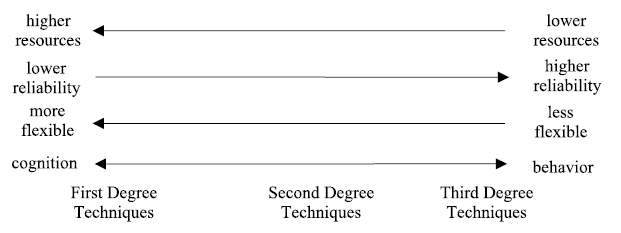
\includegraphics{img/degree_techniques}
\caption{Cost, reliability, flexibility and cognition vs. behavior compared. Source: \cite{Lethbridge2005}}
\label{fig:degree_techniques}
\end{figure}
First degree techniques require more time and effort from both researcher and study participants.
This is due to the fact that they tend to produce a large amount of data that needs processing.
On the positive side of this trade-off, first degree techniques provide the researcher with more flexibility and control over data collection.
Most importantly, first degree techniques allow the researcher not only to understand \textit{how} the task is performed (behavior), but \textit{why} (cognition).
The downside is that the gathered data relies on imperfect human recollection, so care must be taken if complete accuracy of reported facts is important.
Since we are interested in overall cognitive processes instead of minutia, we implement first degree techniques in our case study.

\subsection{Procedures for data collection}
\label{subsec:procedures_for_data_collection}

After having settled on using first degree data collection techniques, in this section we define how the data is to be collected.
This includes a detailed discussion of the user studies that produce the data to collect.

\paragraph{Formative study}~\\
First, a formative study in the form of expert interviews serves to understand scenarios in the patent landscaping task and formulate the requirements. 
The purpose of this first stage of data collection is to acquire subjective, qualitative results since actual human experiences provide valuable insight into benefits and drawbacks of existing solutions. 
Accordingly, \textit{semi-structured} interviews are chosen to understand the users’ mental model of the task.
A semi-structured interview consists of a mix of open and closed questions.
This type of interview is common in case studies \cite{Runeson2009}.
It allows the researcher to follow the natural development of the conversation, improvise and explore the subject at hand while making sure that all relevant topics are addressed.
We discuss the results of the formative study in \autoref{sec:interviews}. 

\paragraph{Ideation}~\\
After the first data collection stage, a concept for the visualization itself must be developed. 
The concept is influenced by the insights gained in the formative study. 
The result of the decisions made at this stage is a digital mockup representing the future interactive prototype (see \autoref{ch:concept} for details).
An implementation phase that follows consists of data preprocessing, applying chosen semantic methods and implementing chosen interaction techniques in a usable interactive prototype (see \autoref{ch:implementation} for details).
After the first proof-of-concept prototype is complete, a short feedback meeting with the potential users takes place .
This helps gather first reactions to the concept and, when necessary, adjust further iterations.

\paragraph{Summative study}~\\
An evaluation of the approach is concluded by the second data collection stage.
The execution of this stage is covered \label{ch:evaluation}.
One of the purposes of the second data collection stage is to uncover cognitive problems and mismatches between the user's mental model of the task and the proposed system.
The second purpose is to evaluate the impact of semantic embeddings as compared to a traditional approach such as \gls{tf-idf} features as document vectors. 
To do that, participants are divided into two groups. 
One group evaluates the traditional approach first and the approach with semantic embeddings afterwards. 
For the second group, the order is reversed.

To gather direct qualitative feedback about usability, a think-aloud study is planned.
The think-aloud approach has its roots in cognitive psychology and is scientifically established \cite{Simon2006} \cite{Ericsson1980}.
It was originally applied in studying short-term memory processes.
Two embodiments of the think-aloud method exist. Ericsson et al.
\cite{ericsson1984protocol} keeps the influence of the experimenter on the outcome to a minimum with rigid procedures.
Contrarily, \cite{Boren2000} et al. approach the experiment as a dialogue.
The participant is still encouraged to talk most of the time.
The researcher mostly listens and acknowledges what is being said, but is allowed to ask questions or intervene in case the participant is lost or a bug in the tested system prevents further progress.
The two techniques were evaluated in \cite{Krahmer2004}.
The outcome shows that the subjects' evaluations were consistent between methods.
However, the subjects completed more tasks and felt less lost with approach from Boren et al.
We therefore choose this embodiment of think-aloud for the qualitative part of our summative study.

For quantitative feedback, we measure the usability score resulting from the use of the prototype.
This helps verify that the visualization based on the proposed approach is easy to use and satisfies the requirements.
For that, \gls{sus} questionnaire \cite{Brooke1996} is chosen.
It is preferred to other questionnaires such as \gls{csuq} \cite{Lewis1993} and \gls{quis} \cite{Chin2003} because it produces reliable results even with small number of participants \cite{Tullis2004}. 
Moreover, it is short, simple and addresses different aspects of user's reaction to the tested system as a whole instead of its specific features.
Alternating positive and negative questions (``I thought the system was easy to use'' vs. ``I found the system unnecessarily complex'') require attention from participants and provide more robust results.
\cite{Laubheimer2018} proposes to combine a \gls{sus} scale with a follow-up question about reasons for the given rating to derive further qualitative insights. 
We follow this suggestion. 

\paragraph{Study subjects}~\\
Experts with experience in patent landscaping from FIZ Karlsruhe serve as subjects of the study. 
According to Nielsen \cite{Nielsen2000}, about 70\% of the insight can be learned from three participants.
Additional participants, especially those after the fifth one, bring merely diminishing returns. 
For this reason, the study is kept small with 3 participants for user interviews and 4 for the think-aloud and \gls{sus} part.

Analysis of the data collected during the second data collection stage allows drawing conclusions regarding the objectives of the study.
Those are described in \autoref{sec:discussion}.

\section{Interviews}
\label{sec:interviews}

Since the formative study defined in the previous chapter had a direct impact on the development of our approach described in \autoref{ch:concept}, we cover the study itself and its results in this section.
First, we describe the organizational and methodological aspects of conducting a semi-structured interview, which is an integral part of the formative study.
After the organizational and methodological aspects follow the descriptions of conversations with patent experts.
We conclude by a summary of how the interviews shaped our understanding of the patent domain and, subsequently, how they influenced the development of a concept for our approach.

\subsection{Procedure}
\label{subsec:procedure}

Three patent experts were interviewed in a semi-structured format as defined in \cite{robson2002real}. 
After greeting the participant, each interview started with some warm-up questions about participant's background. 
Afterwards followed the main part with the most important questions about the domain of patent landscaping itself.
The interview was concluded by cool-down phase with more general questions.
The questions covered relevant aspects of a patent landscaping process such as data quality, usage scenarios and working with different abstraction levels.
A full questionnaire for the interview can be found in \autoref{sec:semi_structured_interview_questionnaire}.

Best practices for conducting user interviews were studied and adopted to the best of interviewer's ability.
Here we list the guidelines that we followed based on \cite{Portigal2013}:
\begin{itemize}
  \item Before scheduling the interview, ask participants if you are allowed to record them talking.
  It is virtually impossible to actively listen and steer the conversation while taking extensive notes.
  An audio recording is usually sufficient.
  Don't forget to check recording equipment before first interview starts.
  \item The questions should not assume a certain point of view. 
  For example, ``How do you feel about X?'' is better than ``Why is X bad?''.
  Ask even if you think you know the answer, you might be surprised.
  \item Show that you understood what the interviewee is saying and ask for clarification. 
  For example, ``You said X, could you please tell me more about it?''.
  \item If questions come up while the interviewee is speaking, don't interrupt them. 
  Write the question down and follow up later.
  \item Speak slowly, don't show hurry.
  If the time is running out, prioritize.
  \item Pay attention to interviewee's body language and try to imitate it when appropriate. 
  Try to prevent defensive poses such as crossed arms.
  \item Leave long pauses after the interviewee's replies.
  Silence is mildly uncomfortable and serves as a prompt to keep talking.
  It also gives the participant a chance for contemplation, allowing them to formulate additions to their last thought.
  \item After the main part of the interview is finished, ask the participant if they have questions for you or would like to tell you something you both had not discussed yet.
  \item After completing the interview thank the participant, stop the recording and note the main topics of the conversation.
\end{itemize}

All participants were to some degree familiar with STN AnaVist, which is an interactive visualization software specifically created for use in the patent domain.
As seen in \autoref{fig:anavist}, it displays a patent map with labeled clusters and allows the users to select an area to compute statistics about the patents in that area as compared to the whole dataset.
Prior exposure to STN AnaVist most probably shaped experts' expectations for a patent landscaping tool.
%Moreover, in their daily work routine the experts use non-visual /move to discussion

The interviews provided valuable insights into workflows and mental processes of patent experts. 
In the the descriptions of the conversations we only elaborate on discussion points that are relevant to the development of our approach. 
The issues not covered here nevertheless significantly contributed to our understanding of the patent domain.

We refer to the participants by the letters of the Greek alphabet and singular ``they'' for both genders to preserve their anonymity.
The grammatical form of singular ``they'' also applies for any (potential) users we mention throughout this work.

\subsection{Participant Alpha}
\label{subsec:participant_alpha}

Participant Alpha has the most experience with patent landscaping.
They composed patent landscape reports and are very familiar with the landscaping tool STN AnaVist and presented it to clients.

Participant Alpha characterized creating a patent landscape as an iterative process. 
It consists of multiple feedback loops that run until converging to a satisfactory result.
 
The first feedback loop involves understanding the needs of the client better. 
It starts when a client commissions a patent analysis and explains their requirements to the expert.
The mutual understanding of the task is difficult to achieve, especially when it evolves based on illustrative results. 
Therefore, after the patent expert presents the client with the result of the current iteration, the client may influence the focus of the analysis.
The expert incorporates the client's suggestions into the further workflow.

The second feedback loop concerns the level of abstraction in the query to the patent database.
Participant Alpha pointed out that the patent attorneys often use very generic vocabulary compared to scientific publications such as papers.
This allows the claimed invention to be protected in a wider variety of embodiments.
Patent offices work against this tactic by demanding a sufficient level of detail to prevent claims from being too broad.
As a result, patent expert sometimes has to experiment with making terms of the search query more or less generic.
If a query consists of parts A, B and C, a combination of generic search terms for A and B and specific terms for C might be followed by a combination of specific terms for A and C with generic terms for B.
Thus, possible combinations of generic and specific terms for parts of the query are tested iteratively until the query result is satisfactory.
The optimal level of detail for each part of the query constitutes a substrategy, and such substrategies are merged in the final query.

Participant Alpha highlighted the importance of uniform names for assignees and inventors. 
They reported a recent ``information flood'' from Asia, especially from China, which necessitates uniform rules for transliterating proper nouns.
According to the participant, uniform names of patent assignees are a distinguishing feature of high-quality datasets that is required by clients.
Non-uniform names make aggregating data, i. e. counting, unreliable.

The participant made a distinction between two kinds of patent landscaping.
One involves looking at a patent set in a quantitative way through the set of metadata attributes.
It helps answer questions such as who are the biggest competitors, since when they have been active, how many applications do they have, in which countries are they active.
The second kind involves better understanding of the technology domain and ability to subdivide it into subdomains.
The participant named freedom-to-operate research as a possible scenario for this kind of analysis.
In this area they saw potential for use of semantic methods such as the contribution of this thesis.

The participant described multiple definitions of a patent family. 
The most widely accepted one and also the broadest one is ``simple family'', which constitutes a group of patents associated with the same priority document.
Simple family may contain patents with claims that differ significantly because they protect different parts of the same invention or take into account regional differences.
Creators of patent databases such as Derwent also create their own definitions of family which are more narrow and typically contain almost identical patents only.

Aside from the freedom-to-operate scenario, the participant also mentioned 1) whitespot analysis, 2) searching for cooperation partners and  3)``licensing out'' patents that are not in company’s core portfolio as valid scenarios where a patent landscaping tool has successfully been used or might be useful.
If one searches for a widespread technology, whitespots can be recognized where a few data points are on their own and not in any big cluster.

Participant Alpha emphasized strongly the importance of data quality. 
They reported that a patent in a full-text database might be about 100 pages long, while same patent in an added-value database, such as Derwent, might be about 2 pages.
This difference is explained by the fact that texts in an added-value database are rewritten by professional writers to a more concise and understandable form.
Added-value databases are used as a default option during a patent search.
Full-text databases are only searched when necessary.

While on the topic of patent classification systems, participant Alpha reported that \gls{ipc} is used by virtually all patent offices worldwide and covers about 98\% patent documents.
Though \gls{cpc} has more meaningful and better structured hierarchy, it is assigned to only 40\% of documents and is therefore unreliable if used by itself.
The participant named subclass level (i. e. A61K), main group (i. e. A61K6) and subgroup (i. e. A61K6/02) as most widely used levels of the \gls{ipc} hierarchy.
Some \gls{ipc} codes are assigned consistently and are suitable for searching using \gls{ipc} codes only, while others require searching with help of key terms. 

\subsection{Participant Beta}
\label{subsec:participant_beta}

Due to their background, this participant has some experience in text mining, especially annotating patent texts.
Accordingly, initial questions led to a detailed discussion on this topic.

Participant Beta pointed out that machine translation, \gls{ocr} artifacts and different writing styles make automatic analysis error prone.
Participant Beta repeated Participant Alpha's assertion about quality of the data playing a crucial role in automated analysis.
The participant elaborated that sometimes the user might get an impression of some trends happening, while in reality they only can be attributed to the noise and errors in the data.

According to Participant Beta, it is difficult to separate citations from the rest of the text, and noise in data occurs when this process was not successful. 
Nevertheless, assuming that citations were recognized successfully, they constitute a very important kind of connection between documents and represent a very strong similarity. 
If A cites B, but they do not have similar key terms, the approach might be faulty.
Patent families should be grouped in an obvious way as well.

Considering usage scenarios, Participant Beta reported that in 80\% of all cases solely the distribution of assignees plotted by publication year was sufficient.
Moreover, participant expressed doubt about value of visual patent landscaping tools compared to traditional non-visual tools.
The participant themselves as well as other patent experts have difficulty interpreting the visual representation of a landscape.
The connection between terms that describe clusters is perceived as far from obvious and needs an explanation.
The meaning of valleys between the mountains in tools such as STN AnaVist is also confusing.
It is unclear to patent experts how one is supposed to recognize patterns and draw conclusions from such representation and what additional knowledge it provides.
Dislike for black-box algorithms was expressed by the participant and their acquaintances.

The participant provided some advice concerning processing of the textual content.

First, they recommended using patent title and abstract together because the title itself might be too short (i. e. one word) or not expressive enough.

Second, they advised to pay special attention to stopword removal. 
There are stopwords that apply for all English texts, such as ``is'', ``have'', etc. 
Stopwords specific to patent domain include structural markers such as ``patent application'', ``description'',  ``prior art'' or``claim''. 
The participant reported that during demonstrations of patent analysis software, they have regularly seen stopwords which should have been removed.

Third, Participant Beta highlighted the importance of not only single-word key terms but phrases that are two or three words long.
Such phrases may consist of nouns but also of adjectives and participles.
However, the participant's impression was that single-word key terms do not appear sufficiently often after key term extraction.
The participant disapproved of this, because some domains possess highly relevant one-word key terms. 
The situation was attributed by the participant to insufficient weighting by the extraction algorithm.

Participant Beta stated that the description field in a patent can be separated into multiple segments such as ``Background of the Invention'', ``Summary of the Invention'', ``Brief Description of the Drawings'', ``Detailed Description of the Preferred Embodiment'' and ``Claims''.
The segmentation is not a straightforward process because the format of the parts of the description varies significantly.
Assuming the segmentation is successful, ``Summary of the Invention'' and ``Detailed Description of the Preferred Embodiment'' provide most value.
The participant expressed curiosity to compare results of a semantic approach between the above-named description segments and ``Background of the Invention''.

\subsection{Participant Gamma}
\label{subsec:participant_gamma}

Participant Gamma had most experience with very specific questions from clients that needed quite specific answers. Typical size of a query result for them is 30-50 patents from which about 5 most relevant have to be selected and presented to the client.

Participant Gamma repeated statements from Participant Alpha about the iterative nature of a patent search. 
They both described the process in a very similar way: one should approach a search from multiple perspectives, develop multiple strategies and merge them at the end.

Participant Gamma explained that freedom-to-operate research needs very complete answers to the search query.
It is very important that no relevant patents are missing from the dataset, otherwise absence of any already protected inventions cannot be proven.

When it comes to working with single patent documents, the workflow is as follows. 
First title and abstract are read. When those are interesting enough, the full text is requested (which might require an additional fee) and studied. 

Participant Gamma echoed Participant Alpha's sentiment about limited usefullness of \gls{ipc} classes. 
For broad analyses they are found helpful, while the more specific the search becomes, the more weaknesses \gls{ipc} shows.

Due to the very narrow nature of requests Participant Gamma works on, they did not see data visualization as the main tool for the search task for them personally.
Instead, they saw it as a way to generate impressive visuals for the stakeholders or other non-experts. 
Nevertheless, they admit that visualization may be useful when dealing with large datasets. 
In this case, interaction and usable filtering features are seen as very important.
Participant Gamma acknowledged that demand for such patent visualization tools exists among their clients.

\subsection{Findings from user interviews and their implications}
\label{subsec:implications}

In this section, we briefly summarize the findings from the user interviews and how they influence our approach:
\begin{itemize}
\item Thematic consistency of IPC classes declines as one moves to the lower levels of IPC hierarchy. 
It also varies a lot depending on the specific technology domain.
One therefore should not expect a clear separation of classes in the semantic space during the clustering (see \autoref{subsec:hierarchical_clustering} for details) and the evaluation (see \autoref{ch:evaluation} for details on evaluation).
Nevertheless, patent experts work with all levels of IPC hierarchy.
\item Names of assignees (companies or individuals a patent belongs to) are often spelled differently throughout the dataset.
This makes grouping patents by assignee name unreliable.
Disambiguated assignee names are one of the characteristics of a quality dataset.
We therefore merge assignees with similar names via fuzzy string matching as a part of the preprocessing before we aggregate the documents (see \autoref{subsec:data_preprocessing} for details).
\item Patent language differs in form and structure from the common written language. 
Both general and very specific vocabulary is used in patent texts, and, accordingly, in patent searches.
Consequently, we use a language model trained specifically on patent texts because it reflects the peculiarities of the patent domain best.
We then attempt to produce generalizations of cluster key terms as described in \autoref{subsec:hierarchical_clustering}.
\item Special attention has to be paid to the elimination of stopwords that add no value to the general understanding. We describe the process of the stopword removal and the stopword lists we use in \autoref{subsec:data_preprocessing} ``Stopword removal''.
\item Patent's title is rarely sufficient to describe its content and thus should be considered together with the abstract. 
The ``Description'' field of a patent consists of segments that vary in relevance and are difficult to separate.
Since our data source does not provide a segmented description, we use another textual field named``Claims'' instead as described in \autoref{subsec:data_preprocessing}.
\item In patent-specific language there are a lot of established expressions that consist of multiple words.
This means it is not sufficient to only extract single-word key terms, which is why we extract both unigrams and bigrams to characterize content of patent documents and document clusters as described in \autoref{subsec:term_extraction}.
\item Belonging to the same patent family constitutes the strongest kind of connection between patents.
In most cases, patents from the same family should be adjacent in the semantic space.
At the same time, families with diverging content exist where this rule of thumb does not apply.
We use proximity of patent families as a minimal criterion which has to be met in the visualization space (see \autoref{subsec:embeddings} for details).
\end{itemize}